\documentclass{article}\author{Hawley, Adam}
\usepackage{amsmath}

\author{Adam Hawley}
\usepackage{graphicx}
\usepackage{wrapfig}
\graphicspath{{./images/}}
\usepackage{gensymb}
\newcommand{\ninth}{\frac{1}{9}}
\usepackage{amssymb}
\title{TEST}
\begin{document}
\tableofcontents
\maketitle{}
\subsection{Admin}
\subsubsection{Exam Format}
One 2 hour exam at the beginning of Spring Term.
\begin{itemize}
\item One question worth 20\% (basic knowledge, shorter questions)
\item Two questions worth 40\% (more advanced, longer questions)
\end{itemize}
{\bf Note: Programming will NOT be examined}
\subsubsection{Reading}
\begin{itemize}
	\item Nielsen, ``Visual Computing: Geometry, Graphics and Vision", Charles River Media, 2005
	\item Prince, ``Computer Vision", Cambridge University Press
\end{itemize}

\maketitle
\section{Lecture 1: Introduction}
\tableofcontents
\newpage

\subsection{Conventions}
\begin{itemize}
	\item Matrices written in uppercase bold eg:
{\bf A} =$ 
\begin{bmatrix}
1&2\\
3&4
\end{bmatrix}
$
\item Matrices are also indexed (row, column) from top left starting at 1.
\item Individual elements are written as lowercase: 
	\\  \centerline{ $ a_{11} = 1, a_{12} = 2, a_{21} = 3, a_{22} = 4 $ }
\item Vectors are simply matrices with a single row or column represented by a lower-case bold symbol:

	\centerline{ $ {\bf a} = 
		\begin{bmatrix}
			x\\y\\z
		\end{bmatrix} OR \ \ {\bf a} = 
		\begin{bmatrix}
			x&y&z
		\end{bmatrix}
	$ }
\end{itemize}

\subsection{Transformations}
\subsubsection{Translation}
Translation involves {\textbf{\textit{component-wise addition}}}.

For example: \\
\centerline{$
\begin{bmatrix}
	x' \\ y'
\end{bmatrix}
=
\begin{bmatrix}
	x \\ y
\end{bmatrix}
+
\begin{bmatrix}
	d_x \\ d_y
\end{bmatrix}
$}
\subsubsection{Scaling}
Scaling involves {\textbf{\textit{multiplication by a scalar}}}.

For example: \\~\\
\centerline{$
\begin{bmatrix}
x' \\ y'
\end{bmatrix}
= s 
\begin{bmatrix}
x \\ y
\end{bmatrix}$}

Or to have a separate dimensional scalars:\\ \\
\centerline{$
\begin{bmatrix}
x' \\ y'
\end{bmatrix} = 
\begin{bmatrix}
	s_x&0\\
	0&s_y
\end{bmatrix} $}
\subsubsection{Rotation}
Rotation involves {\textbf{\textit{matrix multiplication}}}. Using the formula below to give a 2D rotation counter clockwise by angle $\theta$:
\\~\\
\centerline{$
	\begin{bmatrix}
		x' \\ y'
	\end{bmatrix} = 
	\begin{bmatrix}
		\cos(\theta) & -\sin(\theta)\\
		\sin(\theta) & \cos(\theta)
	\end{bmatrix}
	\begin{bmatrix}
		x \\ y
	\end{bmatrix}
$}

Rotation preserves distances: \\
\centerline{$ ||{\bf x}|| = ||{\bf Rx}|| $}\\
\centerline{$||{\bf x}||^2 = x^2_1 + x^2_2 + ... + x^2_n = {\bf x}{\it ^T}{\bf x} $}
\centerline{${\bf x}{\it ^T}{\bf x} = ({\bf Rx}){\it ^T}({\bf Rx}) 
$}
\centerline{${\bf x}{\it ^T}{\bf Ix} = ({\bf x}){\it ^T}({\bf R}{\it ^T})({\bf Rx}) 	
$}
\centerline{$ = {\bf x}{\it ^T}({\bf R}{\it ^T}{\bf R}){\bf x}  
$}
And hence: \\ \centerline{$ {\bf R}{\it ^T}{\bf R} = {\bf I} $} 
\centerline{$ {\bf R}{\it ^T} {\bf R} {\bf R}^{-1} = {\bf IR}^{-1} $}    
\centerline{$ {\bf R}{\it ^T} = {\bf R}^{-1}  $}
So to get the inverse of a rotation you only need to transpose it.
\subsubsection{Affine Transformations}
All of the previously mentioned transformations have been {\bf affine} transformations. These are transformations which can be expressed as matric multiplication and addition: 

\centerline{$ \bf y = Ax + b $} 

For 2D, {\bf A} is a 2x2 matrix and {\bf b} a 2x1 vector.

For 3D, {\bf A} is a 3x3 matrix and {\bf b} a 3x1 vector.  

\subsection{Homogeneous Coordinates}
\subsubsection{Defining Homogenous Coordinates}
Representing the affine transformations can be done by moving from Cartesian to homogeneous coordinates.

All 2D affine transformations can be then represented by a 3x3 matrix (or 4x4 for 3D)

\centerline{$
	\begin{bmatrix}
		x \\ y
	\end{bmatrix}
	becomes
	\begin{bmatrix}
		x \\ y \\ 1
	\end{bmatrix}
$}

\subsubsection{Affine Transformations as Homogeneous Coordinates}
The extra dimension allows uniform treatment of transformations:

Translation: $\begin{bmatrix}x' \\ y' \\ 1 \end{bmatrix}
= \begin{bmatrix}1&0&d_x\\0&1&d_y\\0&0&1\end{bmatrix}
\begin{bmatrix} x\\y\\1\end{bmatrix}$ 

Scaling: $\begin{bmatrix}x'\\y'\\1\end{bmatrix}
= \begin{bmatrix}s_x&0&0\\0&s_y&0\\0&0&1\end{bmatrix}
\begin{bmatrix}x\\y\\1\end{bmatrix}$

Rotation: $\begin{bmatrix}x'\\y'\\1\end{bmatrix}
=\begin{bmatrix}\cos\theta&-\sin\theta&0\\
		\sin\theta&\cos\theta&0\\
		0&0&1\end{bmatrix}
\begin{bmatrix} x\\y\\1	\end{bmatrix}$\\
\vspace{2.5mm}
\vspace{2.5mm}
\\
In general, any affine transformation:

\centerline{$\bf y = Ax + b$}

Can be expressed as:

\centerline{$ \begin{bmatrix}y\\1\end{bmatrix}=
	 \left[ \begin{array}{ccc|c}
	 &{\bf A}&& {\bf b} \\ 0&...&0&1
	\end{array} \right] 
	\begin{bmatrix}
	{\bf x}\\1
	\end{bmatrix}
$}

{\bf Note:} Two homogeneous points are equal if they differ only by a scale factor.
\maketitle
\section{Lecture 2: Transformations}
\newpage

\subsection{Types of Sensor}
There are many different types of sensors used in computer vision:
\begin{itemize}
	\item Optical
	\begin{itemize} \item CCD, Photodiodes, Photomultipliers \end{itemize}
	\item Infra-red (thermal imaging cameras)
	\begin{itemize} \item CCD (Cooled), Photodiodes \end{itemize}
	\item Synthetic Aperture Radar (SAR)
	\begin{itemize} \item Radar, Antenna \end{itemize}
	\item Range Sensors
	\begin{itemize} \item Laser \& Photodiode \end{itemize}
	\item MRI
	\begin{itemize} \item Magnetic field gradients applied causing production of rotating magnetic field which can be measured. \end{itemize}
	\item PET/CAT
	\begin{itemize} \item Simulated radiation emission via magnetic field or radio isotope. \end{itemize}
\end{itemize}
\subsection{From Light to Images}
\subsubsection{Definitions}
\begin{itemize}
	\item {\textit{\textbf {Irradiance}}}: power incident on a surface (power per unit area).
	\item {\textit{\textbf {Radiance}}}: power travelling from a source (power per unit solid angle per unit projected source area).
\end{itemize}
\subsubsection{Charge-Coupled Devices}
The most common device for digitising image information is a charge-coupled device (CCD). 
They are made up of a square array of solid-state capacitors: \\
\begin{figure}[htbp]
	\centering
	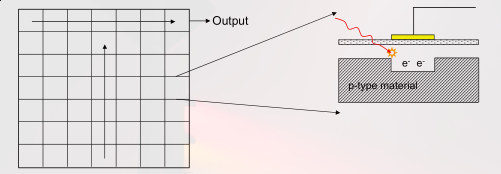
\includegraphics[width=0.9\textwidth]{ccd.png}
	\caption{The flow of electrons inside a CCD}
	\label{fig:CCD}
\end{figure} \\
From the photo-electric effect photons of light knock out electrons from the upper plate and hence charge accumulates in the electron capture ``{\it wells}".
Using a shift register, capacitors transfer their contents to the appropriate neighbour.
The final capacitor dumps the charge for each capacitor into the analogue-digital converter (ADC).
The dump happens once for each capacitor until the contents of each one has been read. \\
\begin{figure}
	\centering
	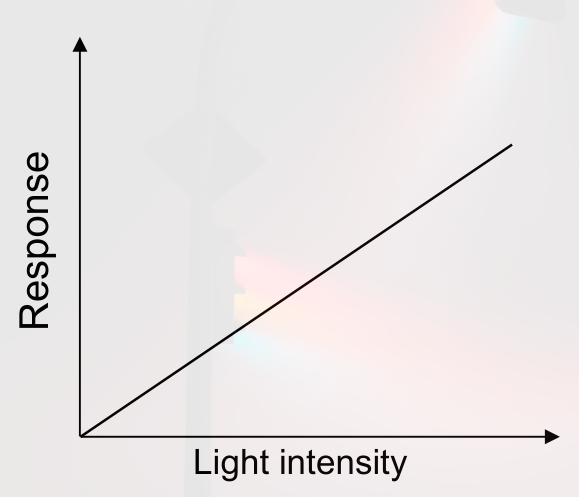
\includegraphics[width=0.3\textwidth]{ccdResponse1.png}
	\caption{Ideal response of a CCD}
	\label{fig:ccdResponse1}
\end{figure}
\\
The ideal reading from a CCD would be as simple as ``$output = gain\cdot input$". See figure \ref{fig:ccdResponse1}.
\begin{figure}
	\centering
	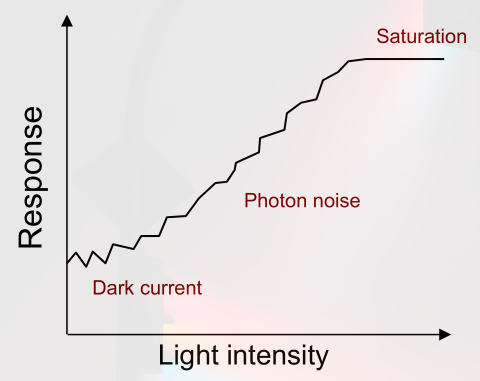
\includegraphics[width=0.4\textwidth]{ccdResponse2.png}
	\caption{Typical response of a CCD}
	\label{fig:ccdResponse2}
\end{figure}
However, a typical reading from a CCD also includes bias and noise (as can be seen in figure \ref{fig:ccdResponse2}).
(``$output = gain \cdot input + bias + noise$'')
The noise mostly comes from the following sources:
\begin{itemize}
	\item Dark Current - Thermal noise.
	\item Photon Noise - Quantum noise.
	\item Quantisation of pixels.
	\item Amplifier
\end{itemize}
\newpage
\subsection{Saturation}
The electron capture wells inside the CCD have a finite capacity $\approx 700 \epsilon ^-/\mu m^2$.
That means that there is roughly a maximum of 100,000 $e^-$ per well in a typical CCD.
When a well is full, the pixel is said to be saturated.
CCDs have a small illumination range (this is what {\it HDR imaging} attempts to overcome).
In an 8-bit image, a pixel brightness of 255 indicates saturation.
\subsection{Noise}
\subsubsection{Signal to Noise Ratio}
The level of noise relative to the signal strength is measured by the {\it signal to noise ratio}. This is often expressed in Decibels (10 times the logarithm of the ratio):
\begin{align*}
SNR (dB) = 10\log _{10}\frac{signal power}{noise power}
\end{align*}

10dB is a tenfold increase in power, 3dB is a doubling of signal power.

\subsubsection{Photon Noise (Shot noise)}
\begin{itemize}
	\item Light sources emit light in photons.
		\begin{itemize}
			\item $\beta$ photons/second on average 
			\item However the photons are emitted randomly.
		\end{itemize}
	\item They follow a Poisson distribution of time t.
		\begin{itemize}
			\item Therefore there is a mean intensity of $\mu = \beta t$
			\item And a standard deviation of $\sigma = \sqrt{\beta t}$
		\end{itemize}
\end{itemize}
Note: At mid-brightness levels the {\it Signal to Noise Ratio}(SNR) for photon noise is around 23dB.

\subsubsection{Dark Current}
{\it Dark Current} is a product of thermal energy from within the CCD.
Electrons are displaced over time that are independent of light actually falling on the sensor (therefore this effect builds up with exposure).
The effect also obviously increases at higher environmental temperatures.
The manufacturing process means certain electron wells may have higher than average dark current ({\it hot pixels}).
{\it Dark frame subtraction} can be used to remove an estimate of the mean pattern of dark current.
However, dark current is also random and hence why it still affects CCD readings.
The randomness of the dark current follows the Poisson distribution just as the photon noise did.

Dark current can be easily shown by taking a picture in complete darkness and inspecting the images to see that it is unlikely that all the pixels will be of absolute darkness.

The SNR for dark current in mid-light levels is approximately 38dB.

\subsubsection{Quantisation noise}
Pixels in photos are digitised to $2^B$ levels. There is a uniformly distributed error on values of $\pm\frac{1}{2}$. This distribution leads to the following properties:
\begin{itemize}
	\item Mean: $\mu = 0$
	\item Standard Deviation: $\sigma =\frac{1}{\sqrt{12}}$ 
	\item $SNR = 10log_{10}(2^{B-1}\cdot \sqrt{12})$
\end{itemize}

$SNR = 26dB$ for 8-bit digitisation, which is better than  the photon noise ratio. Photon noise is the limiting factor of CCDs.
\subsection{CCDs and Colour}
CCDs record photons of all wavelengths, hence they are all monochrome.
A colour image requires red, green and blue values.

To get colour when using a CCD, there are three options:
\begin{enumerate}
	\item Take 3 separate images with a different filter places over the lens. This technique can use filters to allow other frequencies to pass and is hence a multispectral camera. However this method can have issues with motion between frames.
	\item Use a beamsplitter and 3 different CCDs, each with their own colour filter. Using the beamsplitter means that one can have instantaneous colour image capture but careful calibration is required to get exact correspondence between pixels of 3 cameras and it is 3 times more expensive.
	\item Place filters over individual pixels in a mosaic pattern. This is the most common approach. 
		There are more green than red/blue filters since human vision has higher resolution in green than in red/blue. 
		The colours must be interpolated (the process of {\it demosaicing}).
		This method also reduces the effective resolution of the CCD.
\end{enumerate}

\subsection{Conclusions}
\begin{itemize}
	\item Measuring a colour image digitally is difficult
	\item CCDs are generally the best choice
	\item There are many sources of noise, namely:
		\begin{itemize}
			\item Photon noise
			\item Dark current
			\item Quantisation noise
		\end{itemize}
	\item No easy way to capture colour with a CCD
	\item Most common option is a Bayer mosaic
		\begin{itemize}
			\item But this definitely introduces artefacts
			\item (in fact --- these can be used to detect forgeries)
		\end{itemize}
\end{itemize}
\author{Hawley, Adam}
\title{Lecture 3: Photometric Image Formation\\Part 2}

\maketitle
\section{Lecture 3: Photometric Image Formation\\Part 1}
\newpage

\subsection{Brightness}
Light reaches the camera from a scene. 
The amount of light arriving from the scene depends on what is in the scene (strength of light sources, reflectance properties of objects in the scene etc). 
The pixel brightness reported in an image for a given scene radiance quantity depends on the {\it exposure} of the image. 
A camera can control {\it exposure} in a number of ways.

\subsubsection{Formulae}
Before discussing the several parameters which can be adjusted to increase total exposure, there are a couple of formulae to be explained and understood first.

\begin{itemize}
	\item {The amount of light captured by a lens is proportional to the area of the aperture:

\centerline{$Area = \pi(\frac{D}{2})^2$}

D is the diameter of the entrance pupil.}

\item {The {\bf f-number}(N) is the ratio of the focal length (f) to the diameter of the entrance pupil:

\centerline{$N = \frac{f}{D}$}

The higher the f-number, the less light that reaches the CCD (smaller diameter)}

\end{itemize}

Substituting D gets:

\centerline{$Area = \pi (\frac{f}{2N})^2$}

\begin{itemize}
	\item Area is proportional to the reciprocal square of the f-number
	\item Photographers have found it convenient to define a discrete set of f-numbers as ``stops''.
	\item Each stop represents a halving of area of the aperture relative to the previous stop.
\end{itemize}
\begin{align*}
	A_1 &= 2\cdot A_2 \\
	\frac{\pi(d_1)^2}{4} &= 2\cdot \frac{\pi(d_2)^2}{4} \\
	(d_1)^2 &= 2\cdot (d_2)^2 \\
d_2 = \sqrt{(d1)^2\cdot\frac{1}{2}} &= (d_1)\cdot \frac{\sqrt{1}}{\sqrt{2}} = \frac{d_1}{\sqrt{2}}
\end{align*}
Therefore to halve the area of the aperture the f-number must be multiplied by \\ 
\centerline{$\sqrt{2} \approx 1.4$.} \\
Hence, the set of stops is:\\
\centerline{$\frac{f}{1}, \frac{f}{1.4}, \frac{f}{2}, \frac{f}{2.8} ...$}

Each stop represents a halving of the light intensity from the previous stop. 
Hence aperture gives us one way to control how much light reaches the camera.
However, as one changes the aperture, other complex effects are introduced.

As the f-number reduces (aperture gets larger, more light enters lens), ``depth of field'' gets smaller and sharp focus is only possible for a limited range of distances. 


\subsubsection{Aperture}
{\it Aperture} is the first parameter which can change the overall light exposure onto the CCD. 
The {\it aperture} of a camera is the hole through which light travels. 
Aperture size determines the cone angle of a bundle of rays that come to focus in the image plane. 

\begin{itemize}
	\item Small aperture = less light and more highly collimated rays admitted, sharp focus at image plane.

	\item Large aperture = more light and uncollimated rays admitted, sharp focus only for rays with a certain focal length.
\end{itemize}

Aperture sizes are measured in units of {\it stops} with cameras offering a discrete set of aperture sizes.

\subsubsection{Exposure}
Exposure is the accumulated physical quality of light applied to the image-plane over a given time.

Product of the image irradiance (light arriving at the CCD) and time: 
\centerline{$H = E\cdot t$}

{\bf Note:} In practice, cameras apply a non-linear transformation to intensities so the discretised pixel values will be a function of H. However, this is ignored under the {\it ``linear camera''} assumption.

Hence, another way to control how much light reaches the CCD is to change the exposure time.

However, increasing the exposure can cause motion blur and dark current noise (see Lecture 3 notes) will also increase with time.

\subsubsection{Gain}
The brightness of an image can also be increased by passing the analogue signal from the CCD through an amplifier.
The signal gain of a camera is measured on the {\it ``ISO''} scale.
Increasing ISO from its default value of 100 corresponds to increasing signal gain.
Modern CCDs can support incredibly high ISO values and hence operation in very low light.
Remember, increasing the gain will not affect any saturated pixels, they will simply remain saturated.

\subsubsection{Summary}
To summarise, there are three main ways one can increase the brightness of an image:

\begin{itemize}
	\item Increasing the aperture (smaller f-number). (Reduced depth of field)
	\item Longer exposure (motion blur is worsened).
	\item Increasing the gain through a large ISO (noise is also amplified)
\end{itemize}
\subsection{High Dynamic Range Imaging}
\subsubsection{History}
\begin{itemize}
	\item {\bf 1850s}: Gustave Le Gray - Chemical process for combining two exposures.
	\item {\bf 1950s}: ``Dodging and burning'', during film development, make local adjustments to sensitivity.
	\item {\bf 1988-1993}: Technion, Israel --- local tonemapping, first HDR video.
	\item {\bf Modern HDR}: Global HDR {\bf (1993)} --- idea of combining images to compute a global luminance map then tonemap, Debevac et al. {\bf (1997)} --- the method explained below. 
\end{itemize}

\subsubsection{HDR --- How is it done today?}
High dynamic range imaging captures a sequence of images with different exposures. 
Combining the images captures a much wider dynamic range.
The brightness of pixel $i$ in image $j$ is given by:
\begin{align*}
	H_{ij} &= E_i \cdot t_j \\
	\log(H_{ij}) &= \log(E_i) + \log(t_j)
\end{align*}
\begin{itemize}
	\item $t$ is varied for each image
	\item $H$ are the known pixel values
	\item $E$ are the unknown pixel radiances
\end{itemize}

Each image gives us an estimate of the radiance at a pixel.
\begin{align*}
	\log(E_i) = \log(H_{ij}) - \log(t_j)
\end{align*}
The pixel brightness tells us something about how reliable the estimate is:
\begin{itemize}
	\item $\approx 255$ If a pixel is very bright (close to being saturated then the estimate is unreliable.
	\item $\approx 0$ If a pixel is very dark it will be noisy and unreliable. 
\end{itemize}
We give more weight to pixel values near the middle of the range:
\begin{figure}[!h]
	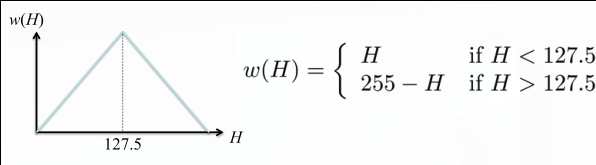
\includegraphics [width=\textwidth]{hdrweights.png}
	\caption{Formula for calculating weights based on pixel value}
	\label{Fig:hdrweights}
\end{figure}
To estimate the true radiance at every pixel we then simply take a weighted average of the estimates from each image:
\begin{align*}
	\log(E_i) &= \frac{\Sigma^K_{j=1}\omega(H_{ij})(\log(H_{ij})-\log(t_j))}
	{\Sigma^K_{j=1}\omega(H_{ij})}
\end{align*}
Saturated pixels are completely excluded. Radiance estimates for a pixel come from images where the exposure is appropriate for the scene radiance.
For colour images, separate channels can be processed independently.

\subsection{Tonemapping}
\subsubsection{Gamma Compression}
{\it Gamma compression} is an effective global (same function applied to all pixels) technique.
\begin{align*}
	I_{tonemapped} = cE^\gamma
\end{align*}
\begin{itemize}
	\item $c$ is a constant scaling where $c>0$.
	\item $\gamma$ is a constant that determines the contrast of the image where $0<\gamma<1$.
\end{itemize}
\subsubsection{Gradient-based Techniques}
The best techniques are local (output colour only depends on the local region around the pixel).
Gradient-based techniques try to preserve local gradient with less concern about overall brightness.
This means that they solve for a set of brightness values that minimises error in gradient while remaining between max and min allowable values.
\end{document}
\title{Lecture 5: About Images}
\author{Adam Hawley}

\maketitle
\section{Lecture 6: Projections}
\newpage

\subsection{Scenes \& Images --- The Basics}
\subsubsection{Intro}
\begin{itemize}
	\item Images represent a projection of the information from a scene in 2D.
	\item Scenes are real in vision, and created in graphics.
\end{itemize}
\subsubsection{What is an image?}
\begin{itemize}
	\item An image is a grid of pixels characterised by image size and pixel values.
	\item Each grey-level image pixel has 8 bits so its value ranges from 0--255. 
	\item Each colour pixel has 3 colour components: red, green and blue.
\end{itemize}

\subsubsection{Histograms}
Histograms represent the {\it the global statistical information} from the image, which may or may not correspond to a specific object. 
They count the frequency of each value in the image.

Histograms are represented as 1-D arrays for grey-level images and as 3-D arrays for colour images - one for each component.

Histogram stretching represents a mapping of the histogram aiming to improve contrast.

\subsubsection{Graphical Objects and 3D}
\begin{itemize}
	\item Voxel representaions can be made by adding layers of images together, producing a volumetric (3D) image.
	\item A {\it graphical object} can be represented as a mesh which is a sequence of vertices joined by polygons (usually triangles).
\end{itemize}

\subsection{Image Production}
\subsubsection{Abstract View}
Stepping back, one can see that image production has four important properties, the latter two of which will be discussed in greater detail later in the notes.
\begin{enumerate}
	\item Images represent projections of real scenes as viewed by the human eye or as taken by a camera.
	\item Images also represent projections of artificially generated scenes in computer graphics.
	\item The theoretical model of vision we use is called the {\it Pinhole Camera}
	\item The more accurate model of real life is known as the {\it Thin Lens Camera}
\end{enumerate}
\subsubsection{Pinhole Camera}

\begin{figure}[h]
	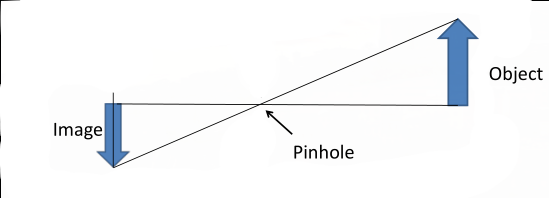
\includegraphics[width=\textwidth]{pinhole.png}
	\label{fig:pinhole}
\end{figure}
The pinhole camera model allows us to use a simplified model of a camera as in figure \ref{fig:pinhole}.
Properties of a pinhole camera:
\begin{itemize}
	\item Continuous sharpness of depth.
	\item Very wide angle range.
	\item Exact perspective projection.
\end{itemize}
{\bf Note:} Pinhole cameras can produce dark images because not enough light enters the camera.

Methods to improve pinhole images:
\begin{itemize}
	\item Increase exposure time (however movement will blur the image).
	\item Increase the size of the pinhole (spread of light causes blurring).
	\item Use lenses to concentrate the light.
\end{itemize}

\subsubsection{Thin Lens Camera}
Real images have lenses which collect light over a finite aperture controlling the amount of light received.
Lenses are charactised by the focal distance $f$ that depends on {\it lens curvature} and {\it lens material}.

{\bf Note:} we discuss single lenses however real cameras use a sequence of lenses.

\subsection{The View Plane}
The {\it View Plane} represents where the image is formed.

In practice the view plane could be any of the following:
\begin{itemize}
	\item Photo-reactive chemicals.
	\item Charge-Coupled Device (CCDs) or CMOS sensors.
	\item Retina in the human eye.
\end{itemize}


\maketitle
\section{Lecture 7: Multiple View Vision}
\begin{itemize}
	\item Prince, Chapter 14 
	\item Nielsen 3.3
	\item Forsyth \& Ponce Chapters 1 and 3
\end{itemize}
\tableofcontents
\newpage

\subsection{Viewing Systems}
In real life we pick up objects, position them and then view them.
In computer graphics objects are positioned in a fixed frame.
The viewer moves to the appropriate position in order to achieve the desired view.

\subsection{Perspective Projections}
We assume that there exists a {\it Centre of Projection} (COP).
Objects' distances from the {\bf COP} cause the objects to appear larger or smaller on the intersecting viewplane. %EXAMPLE 

Lines that are not parallel to the viewplane converge to a vanishing point. 
The {\it Principal Vanishing Point} exists for lines that are parallel to the principal axis.  
This can be clearly seen in the perspective projection of a cube, edges which are parallel to one another appear to converge. %NEEDS EXAMPLE 

\subsection{Parallel/Orthographic Projections}
Here the COP is {\bf always} at infinity.
This means that the viewplane is aligned with the axes and the {\it Direction of Projection} (DOP)

\subsection{View Reference Coordinate System}
\subsubsection{Viewing Parameters}
\begin{itemize}
	\item Location of viewplane
	\item Window within viewplane
	\item Projection type
	\item Projection reference point ({\bf prp})
\end{itemize} 
\subsubsection{Viewplane Parameters}
\begin{itemize}
	\item View Reference Point ({\bf vrp})
	\item Viewplane Normal ({\bf vpn})
	\item View Up Vector ({\bf vup})
\end{itemize}
\subsubsection{Window Parameters}
\begin{itemize}
	\item Width --- $u_{min}$ and $u_{max}$
	\item Height --- $v_{min}$ and $v_{max}$
\end{itemize}
\subsubsection{Coordinate System in Different Projections}
For {\bf Perspective} {\bf Projections} there is only one property:
\begin{itemize} 
	\item {\bf prp} becomes {\bf cop}
\end{itemize}
In {\bf Parallel} {\bf Projections} there are three properties:
\begin{itemize}
	\item {\bf cw} --- The center of window
	\item {\bf dop} --- Direction of projection ({\bf cw} -- {\bf prp})
	\item The projection is {\it Orthographic} if {\bf dop} and {\bf vpn} are parallel
\end{itemize}

\subsubsection{View Volumes for Graphics}
The view volume for perspective projections is a truncated pyramid (frustrum) while the view volume for parallel perspective projections is a cuboid.
The view volumes define a specific region of the scene which is viewed in the current image. 
The view volume is defined by the clipping planes, the projection rays used by the projection system and by the image rectangle.
They are sometimes used in graphics for visualisation such as creating smoke or mist defined only in a specific region of the scene.

\subsubsection{Focal Length in Perspective Projection}
Focal length ($\phi$) is used for two things:
\begin{itemize}
	\item Modelling the effect of the distance to the focal plane
	\item Modelling the density of the receptors (e.g. CCD pixels)
\end{itemize}

\begin{align*}
	x = \frac{\phi u}{\omega} \quad  y = \frac{\phi v}{\omega}
\end{align*}

In practice, the receptors may not be square.
If this case just use different focal length parameters for $x$ and $y$ dimensions:
\begin{align*}
	x = \frac{\phi_x u}{\omega} \quad  y = \frac{\phi_y v}{\omega}
\end{align*}

\subsubsection{Offset}
Currently we assume that (0,0) is where the principal ray strikes the image plane however if this is not the case (and a different coordinate system is used e.g (0,0) in the top left corner) then one can use an offset ($\delta$) or a skew parameter ($\gamma$):
\begin{align*}
	x = \frac{\phi_x u + \gamma v}{\omega}+\delta_x \quad  y = \frac{\phi_y v}{\omega}+\delta_y
\end{align*}
\subsubsection{Intrinsic Parameters}
The aforementioned focal lengths, skew and offset form the set of {\bf intrinsic} {\bf paramters}:
\begin{align*}
	{\phi_x, \phi_y, \gamma, \delta_x, \delta_y}
\end{align*}
It is convenient to store these in an {\bf intrinsic} {\bf matrix}:
$
\begin{bmatrix}
	\phi_x & \gamma & \delta_x \\
	0 & \phi_y & \delta_y \\
	0 & 0 & 1
\end{bmatrix}
$

\subsubsection{Extrinsic Parameters}
If the camera itself is not centered at the origin of the world coordinate system which is often the case. 
If more than one camera is going to be used then it is very common for an arbitrary coordinates system to be used.
To deal with this we express world coordinate points in the local coordinate system of the camera before they are passed to the projection model.
\begin{align*}
	\begin{bmatrix}
		u' \\ v' \\ \omega'
	\end{bmatrix}
	=
	\begin{bmatrix}
		\omega_{11} & \omega_{12} & \omega_{13} \\
		\omega_{21} & \omega_{22} & \omega_{23} \\
		\omega_{31} & \omega_{32} & \omega_{33}
	\end{bmatrix}
	\begin{bmatrix}
		u \\ v \\ \omega
	\end{bmatrix}
	+
	\begin{bmatrix}
		\tau_x \\ \tau_y \\ \tau_z
	\end{bmatrix}
\end{align*}
\centerline{or}
\begin{align*}
	P' &= \Omega P + T
\end{align*}
\subsubsection{3D Transformations}
{\bf $\Omega$} above is the product of 3D transformations where:
\begin{align*}
	\Omega &= R_xR_yR_z
\end{align*}
The same principles apply but now to 4D-homogeneous space.
Rotation is still defined with respect to a specific axis:

\bigskip
\begin{center}$
\begin{array}{l l}
	\mbox{{\bf Axis}} & \mbox{{\bf Positive Direction}} \\
	x & y \rightarrow z \\
	y & z \rightarrow x \\
	z & x \rightarrow y \\
\end{array}$
\end{center}

\begin{align*}
	R_z(\theta) &= 
	\begin{bmatrix}
		\cos\theta & -\sin\theta & 0 & 0 \\
		\sin\theta & \cos\theta & 0 & 0 \\
		0 & 0 & 1 & 0 \\
		0 & 0 & 0 & 1 \\
	\end{bmatrix} \\
	R_x(\theta) &= 
	\begin{bmatrix}
		1 & 0 & 0 & 0 \\
		0 & \cos\theta & -\sin\theta & 0 \\
		0 & \sin\theta & \cos\theta & 0 \\
		0 & 0 & 0 & 1 \\
	\end{bmatrix} \\
	R_y(\theta) &=
	\begin{bmatrix}
		\cos\theta & 0 & \sin\theta & 0 \\
		0 & 1 & 0 & 0 \\
		-\sin\theta & 0 & \cos\theta & 0 \\
		0 & 0 & 0 & 1
	\end{bmatrix}
\end{align*}
\subsubsection{Camera Calibration}
How does one point in the scene relate to the observed point in the image.
A 3D point of coordinates ($X,Y,Z$) from the scene is related to a 2D point ($u,v$) from the image by the equation:

\begin{align*}
\lambda \begin{bmatrix}x \\ y \\ 1\end{bmatrix}
=
\begin{bmatrix}
	\phi_x & \gamma & \delta_x & 0\\
	0 & \phi_y & \delta_y & 0\\
	0 & 0 & 1 & 0
\end{bmatrix}
	\begin{bmatrix}
		\omega_{11} & \omega_{12} & \omega_{13} & \tau_x \\
		\omega_{21} & \omega_{22} & \omega_{23} & \tau_y \\
		\omega_{31} & \omega_{32} & \omega_{33} & \tau_z \\
		0 & 0 & 0 & 1
	\end{bmatrix}
	\begin{bmatrix}u \\ v \\ w \\ 1	\end{bmatrix}
\end{align*}

\maketitle
\section{Lecture 8: Colour Perception}
\newpage

\subsection{Epipolar Geometry}
Considering two pinhole cameras with different projection centres, in order to relate the two images one can use {\it Epipolar Geometry}.

\begin{itemize}
	\item $p_l$ \& $p_r$ are the vectors from the centres of projections $O_l$ in the left and $O_r$ in the right image to the corresponding projections $P_l$ \& $P_r$ of the same 3D point $P$.
	\item $h_l$ \& $h_r$ are called {\bf epipolar lines} --- they are located at the interection between the image plane and the plane formed by the points P, $O_l$ \& $O_r$.
		Each point P will have an epipolar line in each image plane.
	\item $e_i$ \& $e_r$ are epipoles representing the intersection points of $O_l O_r$ with the left and right image planes.
		They may be located outside the actual images.
\end{itemize}


To estimate the epipolar geometry, determine the mapping between corresponding points in the two images.
\begin{align*}
	p_r &= Rp_l + t \\
	O_lO_r &= t
\end{align*}
The left and right images are connected by means of a matrix representing rotation {\bf R} in the plane $PO_lO_r$ and translation {\bf t}.  

Epipolar geometry depends only on the cameras' internal parameters and relative pose.
\begin{align*}
	\text{If } O_lO_r,P_rP,P_lP \text{ are coplanar} \implies \textbf{p}_l\cdot
	\left [\textbf{t} \times (\textbf{Rp}_r) \right ]
	= 0
\end{align*}

This results in the Fundamental matrix.
\begin{align*}
	\textbf{p}^T_r\textbf{Ep}_l \text{ where: }\\
	E = 
	\begin{bmatrix}
		0 & -t_z & t_y \\
		t_z & 0 & -t_x \\
		-t_y & t_x & 0
	\end{bmatrix}
	\textbf{R} \\
	rank(\textbf{E}) = 2
\end{align*}
We have a well defined geometry linking the epipolar vectors of right and left images by means of matrix \textbf{E}.

\subsection{Image Rectification}
Image rectification is implemented by multiplying the image matrices with a geometric transformation matrix.
Epipolar lines become parallel following image rectification.

\subsection{Depth Maps}
Depth maps represent the distance from the image plane to the actual 3D scene.
In computer vision depth maps are estimated from the disparity between pairs of images.
If images are aligned, the disparity represents a displacement along the epipolar lines.

In computer graphics, the depth map (also called \textit{Z-Buffer}) is calculated as the distance from the 3D scene to the image plane.

\subsubsection{Depth Maps for Photorealistic Effects}
Depth maps can be used to apply effects to specific objects/regions of the image.
For example, portrait modes can use depth to apply a blurring effect to everything in an image except for a face.

\subsubsection{Estimating Depth Maps}
Depth maps can be estimated from stereo images based on fields of disparities.
Each disparity represents the correspondence of a block of pixels from one image into the other.
Objects which are far away will be in identical places in both images (disparity is 0).
Objects which are near the camera will have a displacement according to their depth.

\subsubsection{Block Matching}
Comparing the two images and finding the disparities is done using a method called Block matching.
Block matching is done using the following procedure:
\begin{enumerate}
	\item Calculate differences between the block of pixels, pixel-by-pixel, from left image and all blocks from a search region in the right image.
	\item The search region is centred at the location of the original block of pixels.
	\item Choose the block of pixels from the second image which is the most similar with the orignial block and define a vector as the difference of their locations.
\end{enumerate}

The size of the block of pixels $B_x \times B_y$ should not be too small (which may lead to confusion) or too large (requiring large computational complexity and low disparity resolution).
Block matching works well when we have well defined features or non-regular textures.
Block matching does not work well where we have regions of constant colour or regular textures.

\subsubsection{Estimating Depth Maps \romannumeral2}
When estimating the depth maps from real images, local errors emerge due to:
\begin{itemize}
	\item Left and right images are affected by the noise of the image sensors and changes in light.
	\item Results in wrong matches and consequently in errrs in the depth map.
\end{itemize}

\subsubsection{3D from Multiple Views}
Several images are provided from various angles and the 3D scene is reconstructed as made up of voxels.
Surfaces are visible only from some cameras.
For this process, the cameras have to be calibrated.
Usually, this calibration is done using chessboard patterns.

\subsection{Space Carving}
The 3D scene is formed using space carving.
Space carving starts with a cube in the scene.
If there is no projection onto any of the images for that voxel, then it is carved away.Otherwise --- get all pixels where it projects.
Use all of the images to estimate the colour of the voxel from the pixels' colour.

When a voxel is seen from several images a statistical estimation takes place (averaging or median statistics).


\textit{Floating voxels} and uneven surfaces emerge due to wrong correspondences and are caused by:
\begin{itemize}
	\item Confusions in colours due to the illumination and noise
	\item Errors in cameras' geometry due to wrong camera calibration.
\end{itemize}

\subsection{Conclusions}
\begin{itemize}
	\item Stereo vision
	\item Epipolar geometry
	\item Image rectification
	\item Depth maps
	\item Multi-view vision for 3D scene estimation
	\item Space carving method
\end{itemize}

\end{document}

\maketitle
\section{Lecture 9: Colour Image Representation}
\newpage

\subsection{The Light Spectrum}
\subsubsection{Visible Light}
Radiation in nature is characterised by wavelength and frequency.
Visible light has a very narrow wavelength range of 350nm - 780nm (neighbouring to ultraviolet and infrared respectively).

\subsubsection{Visualising Other Spectra}
In order to visualise other spectra, we can use the appropriate sensors and lenses.
For example, visualising infrared radiation has many uses including security and medicine.

Most of the time, we use {\it true colour} to represent radiation as it is what we use in photographs.
However, when visualising other spectra which are not within the reach of true colour, one can use {\it pseudocolour} or {\it greylevel mapping} to represent the radiation.
\begin{itemize}
	\item {\bf Pseudocolour} is when the image uses colours re-assigned according to an LUT or function.
	\item Similarly, {\bf greylevel mapping} represents the radiation using a function however the product of this function represents a grey level value and no colours are involved.
\end{itemize}

\subsection{Hyperspectral Images}
\subsubsection{What Are Hyperspectral Images?}
A {\it hyperspectral image} associates a vector of various wavelengths to a pixel.
This results in volumetric images where one of the dimensions is the wavelength (spectral dimension).
The information in each pixel depends on the capacity of the corresponding object surface to absorb and reflect radiation of that specific wavelength.

Hyperspectral imaging collects and processes information from a large range of wavelengths using specific sensors. %INCLUDE GRAPHIC

\subsubsection{Appplications}
Hyperspectral imaging can be used for a number of things:
\begin{itemize}
	\item Identification of materials by measuring their spectral absorption and reflectance.
	\item Discovery of natural resources by using ground-penetrating images taken from aeroplanes and satellites.
	\item Discovery of concealed objects
	\item Assessing the quality of fruit and vegetables
\end{itemize}

\subsection{Illumination}
Light sources are characterised by their own spectral range $[\lambda_1-\lambda_2]$.
The spectral range interacts with scene colours which means that the output in the image depends on the light spectral range of the light source.
For example, consider the difference between some photos with and without a flash or at different times of day.

\subsection{CIE Colour Model}
\subsubsection{Outlining the CIE}
{\bf Commision Internatinal de l'Eclairage} (CIE).
Three standard primaries $x,y,z$ for representing all colours perceived by humans.

Where {\bf C} is a colour to be matched: 
\begin{align*}
	{\bf C} = X.{\bf X} + Y.{\bf Y} + Z.{\bf Z} 
\end{align*}
This can be thought of as a 3D space.
Chromacity values depend on dominant wavelength and saturation (not the luminance) through normalising ($X,Y,Z$):
\begin{align*}
	x &= \frac{X}{X+Y+Z} & y &= \frac{Y}{X+Y+Z} & z &= \frac{Z}{X+Y+Z}
\end{align*}
Since $x + y + z = 1$ we only need ($x,y$) to specify the chromactiy value, if we want the luminance information then we just need ($x,y$) and $Y$ since:
\begin{align*}
	X &= \frac{x}{y}Y & Z &= \frac{1-x-y}{y}Y
\end{align*}

Aspects of the chromacity diagram:
\begin{itemize}
	\item Interior corresponds to visible colours
	\item Pure colours appear along the curve
	\item {\bf Illuminant C} is considered to be `standard daylight'  
	\item Luminance dependent colours do not appear (e.g brown) 
\end{itemize}

\subsubsection{Selecting Colours Using the CIE}
The diagram allows us to determine the dominant wavelength and {\it excitiation purity} of light:
\begin{enumerate}
	\item Match colour A using the 3 CIE primaries
	\item Plot the position in the CIE chromacity diagram
	\item The mix of two colours lie on a straight line between them
\end{enumerate}
\begin{align*}
	\text{dominant wavelength} &= B \\
	\text{excitation purity} &= \frac{|AC|}{|BC|} \times 100 \%
\end{align*}

Complementay are those that can be mixed to yield white light.
Colours which have no dominant wave-length are referred to as non-spectral.


\maketitle
\section{Lecture 10: Light \& Reflectance}
\newpage

\subsection{Colour Image Pipeline}
\begin{itemize}
	\item Bayer colour filter arrays --- mosaics of colour
	\item Coordinated colour temperature transform (CCT) --- colours are adjusted based on light source illiminating the scene --- based on tables of chromacity for standard illumination
	\item Colour gamut -- depends on a specific device
	\item White balance adjustment
	\item Demosaicing --- interpolates the R,G,B components producing the full colour image
\end{itemize}

\subsubsection{Bayer Mosaics}
Bayer pattern sensors are composed of colour filtered sensors in a specific layout, using two green sensors for each red and blue sensor.

\subsubsection{Demosaicing}
Demosaicing is the process of turning the sensor output with 3 separate colour channels into one pixel per three colour values.
I.e going from 2 greens, 1 red and 1 blue to one pixel which represents them all.

\subsubsection{Colour Matching}
Colour matching functions work by combining red, green and blue to define the colour accuracy.
A particular colour (spectral wavelength) can be matched to filtered measurements of sensor values.
The matching is performed as relative values of colour primaries.
A different sensor could provide different colour values.

\subsubsection{Colour Gamut}
The colour gamut represents the colours which are reproduced by a specific media (the rest of the colours are clipped).
The gamut restrics which colours can be visualised.
Graphics artists should consider the display media gamut for the colours of his graphics.

\subsubsection{CIE}
The CIE chromacity diagram is obtained based on their perception.
Hue is defined on the  border.
Colour saturation decreases as you go towards the centre (location of white).

\subsection{Colour Systems}
\subsubsection{RGB}
The 3 types of cone in the human eyes are sensitive to 3 wavelengths: 630nm (red), 530nm (green) and 450nm (blue).
\begin{align*}
	C_\lambda = R\textbf{R} + G\textbf{G} + B\textbf{B}
\end{align*}
The values for \textbf{R,G,B} are defined by:
\begin{itemize}
	\item Standard NTSC phosphor
	\item Monitor/phosphur manufacturers
\end{itemize}
For two monitors 1 and 2 with different gamuts we can compute:
\begin{align*}
	\begin{bmatrix}
		Y \\ Y \\ Z
	\end{bmatrix}
	=
	\begin{bmatrix}
		X_r & X_g & X_b \\
		Y_r & Y_g & Y_b \\
		Y_r & Y_g & Y_b \\
	\end{bmatrix}
	\begin{bmatrix}
		R \\ G \\ B
	\end{bmatrix}
\end{align*}

\subsubsection{YIQ and CMY}
\paragraph{YIQ}
Composite signal for TV defined by NTSC.
This colour system is based on CIE.
The Y parameter carries luminance (similar to the CIE).
I and Q contribute to hue and purity.
\begin{align*}
	\begin{bmatrix}
		Y \\ I \\ Q
	\end{bmatrix}
	= 
	\begin{bmatrix}
	0.299 & 0.587 & 0.144 \\
	0.596 & -0.275 & -0.321 \\
	0.212 & -0.528 & 0.311
	\end{bmatrix}
	\cdot
	\begin{bmatrix}
		R \\ G \\ B
	\end{bmatrix}
\end{align*}

\paragraph{CMY}
Subtractive colour model used in printing.
Cyan ink subtracts red component of light, magenta subtracts green component and yellow subtracts the blue component of light.
The printing process uses 3 or 4 dots. (CMYK)
\begin{align*}
	\begin{bmatrix}
		C \\ M \\ Y
	\end{bmatrix}
	= 
	\begin{bmatrix}
		1 \\ 1 \\ 1
	\end{bmatrix}
	-
	\begin{bmatrix}
		R \\ G \\ B
	\end{bmatrix}
\end{align*}

\subsubsection{3D Polar Coordinates}
These spaces use a cylindrical (3D polar) coordinate system to encode the following three psycho-visual coordinates:
\begin{itemize}
	\item Hue (Dominant Colour Seen)
		\begin{itemize}
			\item Wavelength of the pure colour observed in the signal.
			\item Distinguishes red, yellow, green etc.
			\item More than 400 hues can be seen by the human eye.
		\end{itemize}
	\item Saturation (Degree of Dilution)
		\begin{itemize}
			\item Inverse of the quantity of ``white'' present in the signal.
			A pure colour has 100\% saturation, the white and grey have 0\% saturation.
			\item Distinguishes red from pink.
			\item About 20 saturation levels are visible per hue.
		\end{itemize}
	\item Brightness
		\begin{itemize}
			\item Amount of light emitted.
			\item Distinguishes the greylevels.
			\item The human eye perceives about 100 levels.
		\end{itemize}
\end{itemize}

\subsubsection{Munsel}
The Munsel colour system is a cylindrically mapped colour system.
\begin{itemize}
	\item Hue: 100 Equally spaced hues around circle
	\item Saturation: Starts at 0 on the centre line and increases to 10-18 depending on the hue
	\item Brightness: 0 for black up to 10 for white
\end{itemize}

\subsubsection{HSV}
The HSV colour system is the most intuitive model for users.
\begin{itemize}
	\item H = Hue (0.0\degree-360.0\degree)
	\item S = Saturation (Ratio from 0.0-1.0)
	\item V = Value (Intensity)(0.0-1.0)
\end{itemize}
The colour system is based on a hexcone shape.
When S=1 and V=1 ``akin to artists pure pigment'':
\begin{itemize}
	\item Hue: Change H
	\item Tints (Adding white): Decrease S
	\item Tone (Adding black): Decrease S and V
	\item Shade: S=1, decrease V
\end{itemize}

\subsubsection{HSL}
\begin{itemize}
	\item Hue
	\item Saturation
	\item Luminance
\end{itemize}
The HSL colour system uses a double cone representation.
Hue is represented 0\degree-360\degree.
Saturation is the value 0-1 out horizontally from the centre.
Luminance has a 0-1 value out vertically from the bottom.

\subsection{Colour Image Histograms}
For the HSL colour system, colour image histograms are generated as follows:
\begin{itemize}
	\item The luminance is quantised into N+1 levels. (E.g 256)
	\item For each level (bin)
\end{itemize}

\subsection{Colour Representation Characteristics}
\begin{itemize}
	\item \textbf{RGB}: Most widely used because of its simplicity. 
	\item \textbf{HSV}: Most intuitive to a computer graphics artist. 
	\item \textbf{CIE Lab}: Most accurate colour system for the human eye. 
	\item \textbf{YIQ}: Best representation of image grey-level is the Y component. 
\end{itemize}

\subsection{Conclusions}
\begin{itemize}
	\item Colour image acquisition
	\item Bayer filters
	\item Colour gamuts
	\item RGB/CMY/YIQ colour spaces
	\item Munsel/HSV/HSL colour spaces
	\item Colour image histograms
\end{itemize}


\maketitle
\section{Lecture 11: Shape-from-Shading}
\tableofcontents
\newpage

\subsection{Light and Reflectance}
Images are produced by light falling on a camera sensor:
\begin{itemize}
	\item The light must come from somewhere
	\item It may be reflected from surfaces before it reaches the camera
\end{itemize}

Hence we need models of:
\begin{itemize}
	\item Light sources
	\item Reflectance of light from surfaces
\end{itemize}

Illuminating a surface gives rise to shading --- very important for realism and the perception of 3D shape.

\subsection{Importance of Shading}

We perceive curved surfaces through their shading patterns.
Shading arises when we add a light source to our scene and employ a reflectance model.

\subsection{Image Formation Process}
Factors that affect the amount of light reflected towards us:
\begin{itemize}
	\item Object shape and in particular the angle of the surface; if the surface is perpendicular to the light from the source it is more likely to reflect light.
	\item Different materials; some materials can give very different reflections of light such as a snooker ball which gives one small concentration of bright reflection compared with velvet which gives a much more even amount of light reflected in a bigger region.
	\item Illumination conditions
	\item Viewpoint/direction, camera parameters.
\end{itemize}

The surface ``reflectance properties'' of an object are described by a {\bf reflectance} {\bf model} (or illumination model). 

\subsection{Distant Vs. Local Illumination}
\subsubsection{Distant Illumination}
Light sources which are very far away (e.g the sun) are often assumed to be at an infinite distance.
This allows for two simplifications:
\begin{itemize}
	\item Direct constant within scene
	\item No attenuation
\end{itemize}
\subsubsection{Local Illumination}
Light sources situated within the scene (local) are more complex:
\begin{itemize}
	\item Direction varies within the scene
	\item Objects closer to the source are illuminated more strongly than those futher away (there is greater {\textbf {\textit {light source attenuation}}})
\end{itemize}

\subsection{Light Source Attenuation}
The physically correct model for attenuation of a light source follows the classical one over distance squared form:
\begin{align*}
	f_{att} = \frac{1}{d^2_L}
\end{align*}
Where $d_L$ is the distance to the light source.

Even though this is physically correct, this sometimes gives too severe a fall off to be used in graphics.
For this reason, alternative functions are sometimes used.
For example:
\begin{align*}
	f_{att} = \frac{1}{d_L}
\end{align*}

\subsection{Point Sources and Spotlights}
The simplest light source type is a {\bf point source}.
Characterised by a 3D location (local) or 3D direction vector (distant) and an intensity or colour.
Sometimes the intensity of a distant light source is encoded in the length of the direction vector.

A {\bf spotlight} is a point source that only emits light in a constrained cone of angles.
For example: studio ``barn door'' type spotlights.

\subsection{Ambient \& Distributed Sources}
{\bf Ambient light} is light that arrives equally from all directions.
This makes it a good model for a cloudy day.
It also leads to very {\it flat} images which lack shading.

{\bf Distributed sources} emit light from an area.
This means that regions may be illuminated by part of the source.
It leads to soft shadows: penumbra around shadowed regions.

\subsection{Environment Maps}
In reality, light arrives at a point from all directions.
One useful approximation iss a spherical {\bf environment map}.
Each pixel is like a distant point source with its own direction and colour.

%CHECK LECTURE TO SEE WHAT WE NEED TO KNOW ABOUT THE RENDERING EQUATION
\section {The Reflectance Equation}
See slides.

\subsection{Local Vs. Global Reflectance}
In practice, light bounces off surfaces onto other surfaces (perhaps many times) before reaching our eye.
If it didn't, then any surface  not directly illuminated would be invisible.
Light reflecting from one surface to another is called {\bf interreflection}.
In this lecture, we consider only {\bf local models of reflectance}.
In this case, we treat each point separately and only consider illumination coming directly from a light source.

\subsection{Reflectance Models}
Designing realistic reflectance models is a large part of current computer graphics research.
Many materials have complex reflectance properties:
\begin{itemize}
	\item Human skin
	\item Fur
	\item Velvet
	\item Hair
	\item Brushed metals
	\item The underside of a CD!
\end{itemize}
A reflectance model describes what happens when light from a certain direction strikes a surface.
When this happens light may be:
\begin{itemize}
	\item Absorbed (As on a \textbf{Translucent Surface})
	\item Scattered (As on a \textbf{Diffuse Surface})
	\item Reflected (As on a \textbf{Specular Surface})
	\item Transmitted into the surface
\end{itemize}
Or any combination of the above.

Almost all surface reflectance models are of the form:
\begin{align*}
	I = f(n,s,v,P)
\end{align*}
Where $n,s,v$ are the three unit vectors describing direction: \textbf{n} - surface normal, \textbf{s} - light source \& \textbf{v} - viewer.
$P$ generalises some other parmeters describing the material properties of the surface.

\subsubsection{Ambient Reflection Model}
The simplest reflectance model assumes completely ambient illumination:
\begin{align*}
I = L_ak_a
\end{align*}
Where $L_a$ is the strength of the light source and $k_a$ is the ambient coefficient ($0<k_a\leq1).$
$k_a$ is our first example of a material property.
In genereal, we will have a value for each of the RGB channels.

This simple ambient model is not realistic.
It is generally added to models because graphics programmers noticed their models looked too dark otherwise and the shading drop off at the edge of objects was too drastic.
It ignores the fact that parts of an object may occlude others, reducing the amount of ambient light that reaches the surface.

(We will see a better model for ambient reflectance later)

\subsubsection{The Lambertian Reflection Model}
The simples model which accounts for changes in intensity due to changes in surfaqce orientatin is the \textbf{Lambertian Model}.
This is based on the idea of a \textbf{perfecttly diffuse reflector}.
The assumption is that if the surface is macroscopically rough, light will be scattered equally in all directions.
Similarly, it may be that the light which enters the surface is scattered internally and re-emerges completely diffused.
This model is good for materials like paper and chalk.

Where the angle between surface normal and light source, $\theta_i$, is the \textbf{angle of incidence}, the Lambertian intensity is simply:
\begin{align*}
	I = L_dk_d\cos(\theta_i)
\end{align*}
Or in terms of vectors:
\begin{align*}
	I = L_dk_d(\textbf{n}\cdot\textbf{s})
\end{align*}
Note: there is no \textbf{v} since diffuse reflection is independant of viewing direction.
In general, we assume that the light source is distant and hence that $L$ is constant over the entire image.

\subsubsection{Specular Reflection \romannumeral1: The Phong Model}
The Lambertian model gives a dull, matte appearance.
Many real surfaces are macroscopically smooth and appear shiny.
Reflection from these sorts of surfaces is known as specular reflectance.
A perfect specualor reflector only reflects light in the direction \textbf{r}.
Imperfect specular reflectors reflect light into a range of directions around \textbf{r}.
So strength of specular reflectance is determined by andle \textbf{r} and \textbf{v}.
\textbf{r} is the reflection of \textbf{s} about \textbf{n}.
So \textbf{r}, \textbf{s} and \textbf{n} lie in the same plane.
\textbf{r} can be found from \textbf{s} and \textbf{n}: 
\begin{align*}
	\textbf{r} = 2(\textbf{n}\cdot\textbf{s})\textbf{n})-\textbf{s}
\end{align*}
The Phong specular model is a simple phenomenological model of specular reflectance for non-perfect reflectors.
The maximum reflectance is observed when $\theta_{spec} = 0$ where $\theta_{spec}$ is the angle between \textbf{r} and \textbf{v}.
Rapid fall-off is determined by the \textbf{shininess coefficient}, $\eta$.
The specular term is therefore given by:
\begin{align*}
	I &= L_sk_s\cos^{\eta}\theta_{spec} \\
	I &= L_sk_s(\textbf{r}\cdot\textbf{v})^\eta
\end{align*}

\subsubsection{Specular Reflection \romannumeral2: The Blinn-Phong Model}
A problem with computing the perfect reflection direction, \textbf{r}, is that \textbf{n} is different for every point on the surface, so we must recompute \textbf{r} for every polygon --- very slow.
There is a common simplification known as the \textbf{\textit{Blinn-Phong Model}}.
Instead of \textbf{r}, use aa vector halfway between the viewer and the light source.
Since we assume \textbf{s} is distant, it is fixed over the image so we only need to calculate \textbf{h} once per image:
\begin{align*}
	\textbf{h} = \frac{\textbf{s} + \textbf{v}}{\|\textbf{s} + \textbf{v}\|}
\end{align*}
If \textbf{n}=\textbf{h}, we have perfect specular direction.

\subsubsection{The Complete Phong Model}
The full Phong model is simply the sum of the ambient, diffuse and specular terms, summing over all lights:
\begin{align*}
	I = k_aL_a + \sum_{lights}(k_d(\textbf{n$\cdot$s})L_d + k_s(\textbf{n$\cdot$h)}^{\eta}L_s)
\end{align*}

\subsection{Colour in Reflectance Models}
In all of the reflectance model equations given so far, material properties (ambient, diffuse, specular coefficients and shininess) are \textbf{wavelength dependent}.
The strength of the light source is also wavelength dependent (i.e light source has a colour).
Some of the latest reflectance models evaluate intensity over the whole visible spectrum.
In practice, we provide RGB values for light sources and ambient, diffuse and specular coefficients.
Often:
\begin{itemize}
	\item Ambient RGB = Diffuse RGB (Object Colour)
	\item Specular RGB = White
\end{itemize}

\subsection{Summary}
What you should know:
\begin{itemize}
	\item Types of light source
	\item The rendering equation
	\item Local reflectance models
	\item The Phong model: Ambient, diffuse and specular reflectance
\end{itemize}


\maketitle
\section{Lecture 12: Image Filtering}
\newpage

\subsection{Human Shape-from-Shading}
Humans can perform shape-from-shading well.
They make assumptions to help solve the problem.

Shape-from-shading is also a ``top down'' process.
High level information about the scene is incorporated into the shape estimation process.
Images are interpreted to be consistent with our prior knowledge of shapes.

\subsection{The Geometry of Surface Reflectance}
Remember: Surface reflectance is described in terms of 3 unit vectors, describing the direction of the surface normal, viewer and light source.
This means that intensity ($I$) is a function of the three unit vectors:
\begin{align*}
	I = f(\textbf{n,s,v,P})
\end{align*}

$P$ here refers to the material properties of the surface.

\subsection{Shape-from-Shading}
Shape-from-shading aims to estimate a surface normal for each pixel in an image, a depth map can subsequently be estimated from the normals.

\subsection{Finding Depth From Illumination}

\subsubsection{Unknown Illumination: The Bas Relief Ambiguity}
With different models, the same image can be created by moving the angle of the light source.
This means that we cannot be sure of the depth.

\subsubsection{The Lambertian Reflection Model  \romannumeral1}
Remember: the Lambertian model describes perfectly diffuse reflectance.
It assumes that light is scattered equally in all directions.
Intensity is given by cosine of angle of incidence:
\begin{align*}
	I &= L_dk_d\cos\theta_i \\
	I &= L_dk_d(\textbf{n $\cdot$ s})
\end{align*}

$k_d$ is the \textbf{diffuse coefficient} where $0<k_d\le 1$ representing the proportion of light that is diffusely reflected by the surface (the rest is absorbed).

In a greyscale image we have one intensity value for each pixel.
A surface normal is a 3D vector, so it is described by 3 values (x, y and z).
But its length is fixed to one.
Hence, it has two degrees of freedom (the two angles of a spherical coordinate representation).
This means that we are left trying to recover two unknowns from one measurement and hence the problem is ill-posed (under constrained).

To try and get around this issue we can make simplifications by assuming:
\begin{itemize}
	\item Diffuse coefficient ($k_d$) = 1 --- A perfect white diffuse reflector
	\item Light source direction is known and light source intensity ($L_d$) = 1
\end{itemize}

\subsubsection{The Convex-Concave Ambiguity}
Even with known light source direction, ambiguity remains. %Add example

SEE SLIDES FOR EXAMPLE

\subsubsection{The Lambertian Reflection Model \romannumeral2}
Under the previously outlined assumptions we have:
\begin{align*}
I = \cos\theta_i
\end{align*}
So we can recover the original angle between the surface normal and the light source:
\begin{align*}
\theta_i = \arccos I
\end{align*}
In other words, the surface normal must lie on a cone whose opening angle is determined by the image brightness.
The problem is transformed to choosing a position on the cone for the normal at each pixel.

\subsubsection{Constraints}
Surface normals at adjecent pixels are not independent.
They must correspond to a real surface.
Surface normals which satisfy this constraint are said to be \textit{integrable}.

Other constraints often used include the following:
\begin{itemize}
	\item \textbf{Smoothness} --- surface normal direction should vary slowly across the surface, with no discontinuities.
	\item \textbf{Global convexity} --- prefer convex interpretation to concave.
\end{itemize}

\subsubsection{The Worthington \& Hancock Algorithm}
The Worthington and Hancock alogrithm uses the cone constraint in an iterative framework.
\begin{itemize}
	\item Initialise normals to on-cone position.
	\item Enforce additional constraint (e.g apply smoothing) resulting in off-cone normals.
	\item Rotate normals back to closest on-cone positions.
	\item Repeat until convergence.
\end{itemize}

\paragraph{Initialisation}
Worthington and Hancock use an itialisation in which the normals line up with the local negative image gradient.
This has the effect of picking the darkest point on the cone.
This idea is consistent with an assumption of convexity.

\subsubsection{Deep Learning}
It should be noted that deep research into the application of deep learning is being undertaken.
Neural networks have produced models which can compute depth maps in milliseconds and using fewer assumptions than we are discussing.
For example they are able to estimate the lighting intensity.

\subsubsection{Shape-from-Shading Images Conclusions}
\begin{itemize}
	\item Shape-from-shading is still an unsolved problem.
	\item Fails on real-world images.
	\item Even on synthetic images, surface can be highly distorted.
\end{itemize}

A more practical alternative is to use \textbf{photometric stereo}.
This involves taking multiple images from the same viewpoint but with varying illumination.
Each image provides a partial constraint on the surface normal direction.
They can all then be combined.

\subsubsection{Photometric Stereo}
Two light source directions gives us two cones and two points of intersection.
Two points of intersection means that there is two possible normal directions.
Three light sources uniquely determines the normal.
However, because of noise, this may not be an exact solution.
This means that in reality it is best to use more than three light sources and not compute it exactly but use something similar to a least squares solution.

One image gives the following equation for each pixel from the Lambertian model equation:
\begin{align*}
	I = L_dk_d(n_xs_x + n_ys_y + n_zs_z)
\end{align*}
We can factor the diffuse coefficient into the normal since these are our unknowns and light source intensity into the light source vector since we know both of these:
\begin{align*}
	I = (k_d\textbf{n})\cdot(L_d\textbf{s})
\end{align*}
In other words, we have a linear equation in the scaled surface normal.
The three unknowns are:
\begin{align*}
	N = {[\bar{n}_x \bar{n}_y \bar{n}_z]}^T
\end{align*}
Hence, we need at least three images.
With three images, we have 3 simultaneous equations for each pixel:
\begin{align*}
	I_1 &= \bar{s}_{1x}\bar{n}_x + \bar{s}_{1y}\bar{n}_y + \bar{s}_{1z}\bar{n}_z  \\
	I_2 &= \bar{s}_{2x}\bar{n}_x + \bar{s}_{2y}\bar{n}_y + \bar{s}_{2z}\bar{n}_z  \\
	I_3 &= \bar{s}_{3x}\bar{n}_x + \bar{s}_{3y}\bar{n}_y + \bar{s}_{3z}\bar{n}_z  
\end{align*}

Subscripts represent image number, bar means the vector has been scaled by diffuse coefficient or light source intensity.
$I$ and $s$ quantities are known, $n$ are unknown.
One can solve for $n$ by rearranging and combining equations solving for:
\begin{align*}
	N = {[\bar{n}_x \bar{n}_y \bar{n}_z]}^T = [k_dn_x k_dn_y k_dn_z]^T
\end{align*}
We form a matrix of the scaled light source vectors.
Assuming we have k images, this will be of dimension k times 3:
\begin{align*}
S = 
	\begin{bmatrix}
		s^T_1 \\
		\vdots \\
		s^T_k
	\end{bmatrix}
\end{align*}
We form a vector of the image intensities over the k images:
\begin{align*}
	I = 
	\begin{bmatrix}
		I_1 \\ 
		\vdots \\
		I_k
	\end{bmatrix}
\end{align*}

Then we minimise the following quantity:
\begin{align*}
	\|\textbf{I}-\textbf{SN}\|^2
\end{align*}
The vecot of unknowns \textbf{N} contains the surface normal scaled by the diffuse coefficients.
We can solve for \textbf{N} using the \textit{pseudoinverse} of \textbf{S}:
\begin{align*}
	\textbf{N} = \textbf{S}^+\textbf{I}=(\textbf{S}^T\textbf{S})^{-1}\textbf{S}^T\textbf{I}
\end{align*}
For both the k image and 3 image version, we can separate out the normal and diffuse coefficient:
\begin{align*}
	k_d &= \|\textbf{N}\| & \textbf{n}=\frac{\textbf{N}}{\|\textbf{N}\|}
\end{align*}

\subsubsection{Summary of Photometric Stereo}
Weaknesses:
\begin{itemize}
	\item Strong assumptions:
		\begin{itemize}
			\item Lambertian Reflectance, specularities not modelled
			\item Single point source lights (known directions)
			\item No shadowing
		\end{itemize}
	\item Estimates normals, not full 3D surface
	\item Photometric stereo requires multipple images with no motion
\end{itemize}
Strengths:
\begin{itemize}
	\item Simplicity (linear model of image formation, geometric cone interpretation)
	\item Dense shape estimate (normal for every pixel in the image)
	\item Photometric stereo estimates both albedo and shappe, allowing \textbf{relighting} (rendering with novel light source directions)
\end{itemize}

\subsection{Conclusions}
What you should know:
\begin{itemize}
	\item What shape from shading is
	\item Lambertian reflectance = cone constraint
	\item Worthington and Hancock algorithm
	\item Photometric stereo
\end{itemize}
\maketitle
\section{Lecture 13: Drawing Lines \& Detecting Edges}
\begin{itemize}
	\item Forsyth \& Ponce Chapter 7
\end{itemize}
\tableofcontents
\newpage

\subsection{Intoduction: Images as Functions}
An image can be seen as a function which is discretised and quantised to [0-255] levels.
%INSERT EXAMPLE
The function depends on the scene represented, light properties, image acquisition and so on.

\subsection{Image Subsampling}
Image subsampling consists of removing rows and columns from the image.

Noise is often lost through subsampling because noise is pixel values that are vastly different to their neighbours which do not represent small details.
These pixels are removed through subsampling.
This method is used commonly in deep learning and neural networks because large images require high levels of processing power and time.

When you zoom in on subsampled images, blurring is created, features related to noise and small details are lost.
This is because when you zoom in, pixels are duplicated to fill the new pixels which come from the increase in size.

\subsection{Image Interpolation}
\subsubsection{What is Image Interpolation?}
A better method for restoring the original image after subsampling is to use \textbf{image interpolation}.
\textbf{Image interpolation} uses neighbouring pixels to estimate the original pixel value between the neighbours.

\subsubsection{How is it done?}
The simples example would be to replicate a neighbouring pixel.
However, this is the same as zooming in on the image.
Instead it can be better to take an average of the neighbouring pixels.
\begin{itemize}
	\item \textbf{Bilinear interpolation} considers a weighted average of a 4x4 pixel neighbourhood.
	\item \textbf{Bicubic interpolation} considers a weighted average of an 8x8 pixel neighbourhood. 
	\item \textbf{Adaptive interpolation} depends on image context.
\end{itemize}

\subsection{Image Convolution}
\textbf{Image convulation} uses a window of a neighbourhood.
Kernel $w(x,y)$ with values for each window element.
Calculates the output using the following formula:
\begin{align*}
	g(x,y) = \sum^K_{s=-K}\sum^K_{t=-K}w(s,t)f(x+s,y+t)
\end{align*}
Applying this formula assigns the output to the central element of the $2K+1 \times 2K+1$ window.
Afterwards, the centre moves to the next neighbourhood according to the following:
\begin{align*}
	s &= 1,..., image\_width-1 \\
	t &= 1,..., image\_height-1
\end{align*}

\subsection{Applications of Image Convolution}
\begin{itemize}
	\item Filtering for removing noise
	\item Sharpening images and image features such as object edges and texture
	\item Producing graphical artistic effects in images for \textit{softening} and \textit{sharpening} images, ``fire'' effects and embossing images.
	\item Colouring images as vectors.
\end{itemize}

\subsection{Image Filtering}
Image filtering can be usually applied simply by convolution with a filter mask.

\subsubsection{The Mean (Averaging) Filter}
Consider the convolution of an image with the follwing kernal for a $3 \times 3$ window:
\smallskip
\centerline{$
\begin{bmatrix}
	\ninth & \ninth & \ninth \\
	\ninth & \ninth & \ninth \\
	\ninth & \ninth & \ninth
\end{bmatrix}
$}
The output is the average of the 9 pixels.
This results in the removal of noise but also blurring of the image.

\subsubsection{Gaussian Filter}
The Gaussian filter represents a weighted averaging filter, where the weights are higher in the central region of the window according to the Gaussian equation:
\begin{align*}
G(x,y) = \frac{1}{2\pi\sigma^2}e^{-\frac{x^2+y^2}{2\sigma^2}}
\end{align*}
Note: in graphics, $G$ is discretly approximated. 

\subsection{Image Noise}
Noise occurs naturally in images due to the camera sensors --- increase camera sensitivity (ISO) --- increase noise.
Noise can be removed by filtering.

\medskip
\begin{align*}
	\hat{f}(x,y) = f(x,y) + n(x,y)
\end{align*}
Where $\hat{f}$ is the noisy image, $f$ is the original image and $n$ is the noise itselve.
We can test various filters by artificially adding noise to the image and filtering it afterwards.
\subsubsection{The Mean  Filter}
Images are invariably noisy --- for example when increasing ISO we achieve better detail and better night images --- but also it adds noise to images.

Averaging corresponds to a low pass filter and removes some of the noise by smoothing.
On the other hand averaging filters lead to blurring and can remove small details.
It is also very effective in temporal image sequences.

Problems with the mean filter:
\begin{itemize}
	\item Blurs edges and details in the image
	\item Not effective for impule noise (\textit{Salt-and-Pepper})
\end{itemize}

\textbf{\textit{Salt-and-Pepper Noise}}:\\
Add extreme values to the image of black (0) and white (255) according to a certain percentage.

\subsubsection{Median Filter}
The \textbf{median filter} ranks the data inside the window and picks the middle value.

Note: since the median filter simply takes the middle value of the window, it does not need to be a square image.

\subsection{Rank Order Statistics Filters}
Rank order statistics filters rank the values from the window and pick the value of a certain rank.
The most common rank order statistics filters used are minimum and maximum filters --- these can be used for segmenting the image. 
(See section \ref{maxmin})

\subsection{Maximum \& Minimum Filters} \label{maxmin}
\subsubsection{Maximum Filter}
The max filter takes the maximum value in the neighbourhood.
This has the effect of enhancing bright areas.

\subsubsection{Minimum Filter}
The min filter takes the minimum value in the neighbourhood.
This has the effect of introducing darkness in the image.

\subsection{Conclusions}
What you need to know:
\begin{itemize}
	\item Image interpolation
	\item Image convolution
	\item Image neighbourhoods
	\item Mean filter
	\item Median filter
	\item Gaussian and salt-and-pepper noise
	\item Min and max filters
\end{itemize}



\maketitle
\section{Lecture 14: Shadows \& Interpolation Shading}
\subsection{Pixels}
The pixel space is a rectangle on the $x,y$ plane, bounded by $0\le x\le x_{max}$ and $0\le y\le y_{max}$
Each axis is divided into an integer number of pixels, $N_x$ and $N_y$. The pixels therefore have width and height:
\begin{align*}
	W &= \frac{x_{max}}{N_x} \\
	H &= \frac{y_{max}}{N_y}
\end{align*}

Pixels are reffered to using integer coordinates, that either refer to the locatin of their left hand corners or their centres.
Knowing the $W$ and $H$ values allows the pixel to be defined.
Assuming that $W$ and $H$ are equal, the pixels are square.

\subsection{Line Rastersation}
Straight lines are described by the equation:
\begin{align*}
y = mx + c
\end{align*}

To draw a line we have to vary $x$ between a given range of values and compute a point $y$ at each location according to the line equation.
{\bf Rasterisation} is the process of converting the drawing to pixels in images (also called scan conversion).

\subsection{The Digital Differential Analyser Algorithm}
The Digital Differential Analyser Algorithm (DDA) is an algorithm used to do line rasterisation.
Assuming that we have two endpoints:
\begin{align*}
 p_0 &= (x_0,y_0) 
     &p_1 = (x_1,y_1)
\end{align*}
The point of intersection is given by the line rule where:
\begin{align*}
	m = \frac{y_1-y_0}{x_1-x_0}
\end{align*}
We can consider a point ($x,y$) on the line and then the next point is ($x+1,y+m$) when the line is drawn to the right.

The drawback of the DDA is that it uses folat and rounding operations for each point which require increased computational power.

\subsection{Bresenham's Algorithm}
The DDA algorithm needs to carry out a floating point addition and a rounding operaiton for every iteration.
Bresenham's algorithm operates only on integers requiriing only that the start ad end points of a line segment are rounded.

Firstly assuming that $0\le m \le 1$ and pixel ($i,j$) is the current pixel.
The value of $y$ on the line $x=i+1$ must lie between $j$ and $j+1$.
Because the gradient is in the range 0-$45\degree$ the next pixel must be either East ($i+1,j$) or North East ($i+1,j+1$).
We should also assume that pixels are identified by their centres.

At this point, we have a decision problem, and so must find a decision variable that can be tested to determine which pixel to colour.
First rewrite the equation of a straight line:
\begin{align*}
	y = mx + &c \\
	mx - y + c &= 0 \\
	\frac{\Delta y}{\Delta x} x - y + c &= 0 \\
	F(x,y) = x \Delta y - y\Delta x &+ B = 0
\end{align*}
The useful properties of this function are as follows:
\begin{itemize}
	\item $F(x,y)>0 \implies$ point is above the line
	\item $F(x,y)<0 \implies$ point is below the line
\end{itemize}

The function $F(x,y)$ clearly has the properties required of a decision variable.
Now all we have to do is apply it.
This will involve using rational numbers in the derivation even though we were supposed to be working with integers.

Consider an arbitrary pixel ($x_p,y_p$) that is on a line segment.
We need to test a point to determine which of the possible next 2 pixels to colour.
A suitable point is ($x_p+1,y_p+\frac{1}{2}$) this will be on the vertical boundary between pixels E and NE and at the horizontal midpoint.

\smallskip
If a $F(x_p+1,y_p + \frac{1}{2}) \le 0$ the next pixel is E.
Else, the next pixel is NE.
This is still under the same assumption that that $0\le m\le1$.

Examining the next step we see it is not independent of the decision we have just made.
\begin{itemize}
	\item If E was chosen then the next test will be $F(x_p+2,y_p+\frac{1}{2})$
	\item Else is NE was chosen then the next test will be $F(x_p + 2, y_p + \frac{3}{2})$.
\end{itemize}
Now let $d_n = F(x_p + 1, y + \frac{1}{2})$ and substitute the values $x+2, y+\frac{1}{2}$ and $y+\frac{3}{2}$ back into the definition of $F$ and we have:
\begin{itemize}
	\item If E was chosen then the next test will be $d_{n+1} = d_n+\Delta y$
	\item Else if NE was chosen the next test will be $d_{n+1} = d_n + (\Delta y - \Delta x)$
\end{itemize}

\subsection{Edge Detection}
Edges can be caused by:
\begin{itemize}
	\item Boundaries of objects
	\item Depth discontinuity
	\item Illuminating discontinuity
	\item Shading discontinuity
	\item Margins of shadows
	\item Textures (regions of medium or high variation)
	\item Noise 
\end{itemize} 

\subsubsection{Image Gradient}
The gradient of an image:
\begin{align*}
	\Delta f &= [\frac{\delta f}{\delta x},\frac{\delta f}{\delta y}]
\end{align*}
Edge orientation:
\begin{align*}
	\theta = tan^{-1}(\frac{\delta f}{\delta x}/\frac{\delta f}{\delta y})
\end{align*}
Edge strength:
\begin{align*}
	\|\Delta f\| = \sqrt{(\frac{\delta f}{\delta x})^2+(\frac{\delta f}{\delta y})^2}
\end{align*}
%Need to watch lecture to make further notes


\maketitle
\section{Lecture 15: Global Illumination \& Image-Based Lighting}
\newpage

\subsection{Shadowing}
There are two ways a point can be in a shadow:
firstly, points can be in shadow because they face away from the light source or they can be in darkness caused by another point.
The first is called an self/attached shadow while the second is a cast shadow.

\subsubsection{Self-Shadowing}
How can we test for self shadows?
The check is based on whether the angle between the surface normal and the light source is greater than 90\degree:
\begin{align*}
	\theta_i > 90\degree \implies \text{Self shadow}
\end{align*}
Equivalently, check whether the dot product is negative:
\begin{align*}
	\textbf{n}\cdot\textbf{s}<0 \implies \text{Self shadow}
\end{align*}
This is a very efficient process as it depends on local information only.
Normals are already computed for the reflectance calcultion, simply check dot product.

Self shadowing can be incorporated into the Lambertian model since Lambertian shading uses the same calculation.
(The dot product between the surface normal and the light source)
To make use of the pre-calculated dot product, simply clamp negative values to zero:
\begin{align*}
	I = max(0,\textbf{n}\cdot\textbf{s})
\end{align*}
Note: we did not consider this in either the shape-from-shading or photometric stereo algorithms in the previous lecture.
So self shadows are not accounted for.
``Add noise to the solution'' %CHeck lecture

\subsubsection{Cast Shadows}
Case shadows are much more difficult to calculate.
A point can be shadowed by a distant part of the surface.
(They depend on global geometry)
To check whether a point is in shadow, we must consider all other points on the surface.

If we set height values for every pixel ($x,y$) as $z(x,y)$.
Then the cast shadow test can be written as:
\begin{align*}
	\forall d \in \mathbb{R}^+, z(x,y) + ds_z > z(x+ds_x, y+ds_y) \implies \text{Not in cast shadow}
\end{align*}
For general polygonal surfaces it is more complex:
For every polygon or vertex, compute equation of line to light source.
Then test whether the line intersects any other polygon in the scene e.g:
\begin{itemize}
	\item Compute plane equation for every polygon
	\item Compute line/plane intersection
	\item Test whether intersection is inside or outside extent of polygon
\end{itemize}
There are efficient ways to calculate this.
%Check lecture

\subsection{Flat Shading}
For each planar polygon we compute the surface normal.
The surface normal is constant over the polygon and used to compute a single colour for the polygon.
The whole polygon is then filled with this colour.
For objects which consist of only planar surfaces, it can look fine.
However it generally looks bad for polygonal approximations to curved surfaces.

Flat shading has a very bad effect with curved surfaces.
\textbf{Mach banding} caused by \textbf{lateral inhibiion} means that the human eye effectively has a built in edge detector.
Perception of change in intensity exaggerates actual change.

To smoothly vary the colour of a polygon across the surface we compute a surface normal for each vertex.
The meaning of the normal direction to a point is not well defined so there are two options:
\begin{itemize}
	\item If the surface is described by a parametric function (e.g a sphere or cylinder), just \textbf{derive an analytical expression for the surface normal} from the function.
	\item If the surface is an arbitrary polygonal mesh, compute \textbf{one normal per polygon and combine} these in some way to find vertex normals.
\end{itemize}

\subsection{Face Normals}
Typically, a surface is represented by a list of vertices and a list of faces.
Faces are specified such that vertex ordering is clockwise or counterclockwise when viewed from outward facing side.
To compute a normal to a face, use the cross product of two edge vectors:
\begin{align*}
	\textbf{n} = \textbf{e}_1 \times \textbf{e}_2
\end{align*}

\textbf{Remember}: The length of \textbf{n} gives twice the area of the triangle.
To find \textbf{n} as a unit vector simply divide it by its magnitude.

\subsection{Vertex Normals}
A vertex normal is a combination of the surface normals of the facets adjacent to the vertex.

To find a vertex normal, one can find the average of the surrounding facet normals.
Often a weighted average is used --- weights are areas of facets.
Normals of larger facets contribute more to the vertex normal.
If we use the unnormalised cross products of facet edges, we get this weighting for free.
This method is fine for most purposes but there are more complex methods justified by differential geometry.

\subsection{Interpolation Shading}
There are two main approaches to use vertex normals for interpolation shading:
\begin{itemize}
	\item {\bf Gouraud}: calculate a colour for each vertex, {\bf interpolate colours} along the polygon edge, then interpolate along scanlines within polygons.
	\item \textbf{Phong}: interpolate the vertex normals along the polygon edge, then {\bf interpolate normals}
\end{itemize}

\subsubsection{Drawbacks of Interpolation Shading}
There are two main drawbacks of interpolation shading:
\begin{itemize}
	\item The polygonss are still flat and so the silhouette of curved objects can visibly consist of straight lines.
	\item Shading is carried out after the projection transformation is applied. So if a perspective transformation is used the non-linear transformation of the Z axis may produce odd effects.
\end{itemize}
Both of these effects are reduced by using smaller polygons (i.e a higher resolution mesh).

Other possible problems include strange effects if the normals are set up wrongly.
Mach banding may still be visible --- although colours along polygon edge now match, the rate of change of colour may change drastically giving the appearance of an edge.

\subsubsection{Gouraud Shading}
Summary:
\begin{enumerate}
	\item Each vertex has a surface normal and material properties, pass the reflectance model to compute a colour.
	\item The colouring along the edge of each polygon is interpolated along the edge.
	\item When the polygon is scan converted, interpolate between colours at edge along scanline.
\end{enumerate}

\paragraph{Drawbacks of Gouraud Shading}
The weakness of Gouraud shading is that it assumes the intensity changes smoothly within a polygon.
Specular reflections cause large changes in intensity over a small distance.
If the size of the specularity is small compared to the size of the polygon, Gouraud shading will miss it --- this results in strange behaviour.

\subsubsection{Phong Shading}
In Phong shading we \textbf{interpolate surface normals}.
The reflectance model will be evaluated independently for each pixel.
\begin{enumerate}
	\item Interpolate normals along the polygon edges
	\item Interpolate normals along scanlines, giving a normal for each pixel.
	\item Calculate the colour intensity for each pixel.
\end{enumerate}

\paragraph{Advantages \& Disadvantages of Phong Shading}
Advantages:
\begin{itemize}
	\item Correct specular highlight
	\item Reduced Mach banding problems
\end{itemize}

Disadvantages:
\begin{itemize}
	\item Expensive to compute
\end{itemize}

In modern GPUs something very similar to this happens in pixel or fragment shaders.

\subsection{Conclusions}
What you should know:
\begin{itemize}
	\item Shadows: Cast vs. Self
	\item Face/Vertex normals and how to calculate them
	\item Purpose of interpolation shading
	\item Gouraud vs. Phong Shading
\end{itemize}


\maketitle
\tableofcontents
\newpage

\subsection{Introduction}
Up until this lecture, we have only been modelling illumination in purely local terms.
Reflected intensity is a function solely of light arriving at a point directly from light sources.
\textbf{Global illumination} aims to model all illumination which has arrived at a point including light which has been reflected or refracted by other objects.

\subsection{Global Interactions}
The general approach to considering global interactions:
\begin{itemize}
	\item Start with the light source and follow every ray of light as it travels through the environment.
\end{itemize}
Stopping under any of the following conditions:
\begin{itemize}
	\item Light hits the eye point
	\item Light travels out of the environment
	\item Light has its energy reduced under an admissable limit due to absorption in objects.
\end{itemize}
This process is known as \textbf{\textit{photon mapping}}.
This is computationally very expensive
Certainly not practical for real time graphics but is used offline.

\subsection{Types of Interactions}
Diffusely radiated light reflected off another diffuse surface is called \textbf{Radiosity}.
Specular radiated light reflected off another specular surface is called \textbf{Ray Tracing}.

\subsection{Ray Tracing}
\subsubsection{Whitted Ray Tracing}
The following outlines Whitted ray tracing:
\begin{itemize}
	\item Traces light rays in the reverse direction of propogation from the eye back into the scene towards the light source.
	\item Spawn reflection rays and refraction rays for every hit point (recursive calculation).
\end{itemize}
Global illumination model (specular) and a local model.
Considers diffuse-reflection interactions but not diffuse-diffuse interactions.

Whitted's illumination equation:
\begin{align*}
	I = k_aL_a + \sum^m_{i=1}f_{att_i}L_i[(k_d(\textbf{n}\cdot\textbf{s}_i)+k_s(\textbf{n}\cdot\textbf{h}_i)^{\eta})] + k_rI_r + k_tI_t
\end{align*}
This equation consists of the standard Blinn-Phong model combined with two extra terms; describing reflected light and transmitted light.
These two additional terms contain the recursive elements.

%CHECK LECTURE SLIDES FOR RAY TRACING PSEUDOCODE 

\subsubsection{Problems with Ray Tracing}
Ray tracing, in its current state has several disadvantages:
\begin{itemize}
	\item Shadow rays usually not refracted
	\item Numerical precision --- false shadows
	\item Simplistic model of ambient light
	\item Expensive to compute --- lots of ray-surface intersection computations
\end{itemize}
Note: issues with numerical precision can be alleviated using multiple rays per pixel or sub-pixel jitter --- gives soft shadows.

\subsection{Image-Based Illumination}
Ray tracing allows us to more realistically model how light is transferred around a scene.
This gives a big improvement in realism.
But modelling of the scene (objects+illumination) is a very laborious process.
Humans perceive material properties and shape better under \textbf{natural illumination}.
The easiest way to measure natural illumination is to take a photograph using a mirrored ball (light probe).
The mirrored ball measures incident illuminatin from every direction.
The next step is to resample the picture to ``equirectangular mapping''.
This is called an \textbf{environment map}.
The mapping has two dimensions: elevation ($y$) and azimuth ($\sim x$)

To convert ($x,y$) coordinates to angles:
\begin{align*}
\theta(x) &= \pi\left ( \frac{2x}{x_{max}}-1\right ) \\
	\phi(y) &= \frac{y\pi}{y_{max}}
\end{align*}
To convert angles to a direction (unit vector):
\begin{align*}
	\textbf{s}(x,y) = 
	\begin{bmatrix}
		\sin(\phi(y))\sin(\phi(x)) \\
		\cos(\phi(y)) \\
		\sin(\phi(y)) \cos(\phi(x))
	\end{bmatrix}
\end{align*}
Each pixel (x,y) in an environment map $I(x,y)$ corresponds to a light source with direction \textbf{s}(x,y) and colour $I(x,y)$
To render with an environment map, we just sum over light sources (every pixel in environment map image!) as in Lecture 10.

\subsection{Environment/Reflection Mapping}
Very cheap approximation to appearance of mirror specular object under environment illumination.
Reflect viewing direction about surface normal giving specular lighting direction:
\begin{align*}
	\textbf{s} = 2(\textbf{n}\cdot \textbf{v})\textbf{n}-\textbf{v}
\end{align*}

Use this to look up colour in environment map and copy to pixel.
Environment map stored as texture on reference object such as sphere or cube.
Possible in real time at very low computational cost.

\subsection{Occlusions}
A point on a surface will not necessarily be able to see all of the environment.
i.e Point may be shadowed from certain sources.
Half will be excluded because of self shadowing.
Only those in ``upper hemisphere'' considered.

To handle occlusions exactly, every direction from every surface point needs checking --- like ray tracing with thousands of light sources.

Alternatively: \textbf{precompute} proportion of hemisphere that is occluded and use with environent lighting.
This is \textbf{ambient occlusion}.

\subsubsection{Ambient Occlusion}
\begin{itemize}
	\item Ambient occlusion = 1: Completely unoccluded --- use all sources in upper hemishphere.
	\item Ambient occlusion = 0: Completely occluded --- no light reaches point
\end{itemize}
The \textbf{bent normal} is the average unoccluded direction.

Ambientt occlusion is exact for an environment of perfectly ambient light.
It gives rise to a different kind of shading that is important in human perception.

To use ambient occlusion with general environment lighting:
\begin{enumerate}
	\item Render surface while ignoring occlusions
	\item Downweight resulting intensities by ambient occlusion amount
	\item Use bent normal instead of surface normal
\end{enumerate}
The bent normal is used to describe the dominant direction from which light arrives.
It can be unrepresentative when there are ``\textit{blockers}'' in the scene.

\subsection{Photon Mapping}
Photon mapping approximates the full rendering equation.
Considers all types of interaction and can support image-based lighting.
Based on the \textit{Monte Carlo} simulation:
\begin{enumerate}
	\item Fire photon from light source.
	\item When photon strikes a surface, randomly select a behaviour according to a probabilistic model (e.g. may be absorbed, may be reflected).
	\item Count number of photons that strike each pixel.
\end{enumerate}
The more photons we fire, the better the approximation.
Can include arbitrarily complex models of photon behaviour when striking a surface (e.g. subsurface scattering through multiple layers of a surface).
Can incluse wavelength-dependent effects.

\subsection{Conclusions}
What you should know:
\begin{itemize}
	\item What is global illumination
	\item Recursive ray tracing
	\item Image-based lighting
	\item Ambient occlusion
\end{itemize}

\end{document}
